\documentclass[12pt]{article} 
\usepackage{amsmath} 
\usepackage[dvips]{graphicx}
\usepackage{multirow} 
\usepackage{multicol}
\usepackage{geometry} 
\usepackage{pdflscape}
\usepackage[labelfont=bf]{caption} 
\usepackage{setspace}
\usepackage[running]{lineno} 
% \usepackage[numbers,sort]{natbib}
\usepackage[round]{natbib} 
\usepackage{array}
\usepackage[table]{xcolor}

\newcommand{\methods}{\textit{Materials \& Methods}}
\newcommand{\SI}{\textit{Appendix}~}

\usepackage{titlesec}

\titlespacing*{\section}{0pt}{-0\baselineskip}{-0\baselineskip}
\titlespacing*{\subsection}{0pt}{-0\baselineskip}{-0\baselineskip}
\titlespacing*{\subsubsection}{0pt}{-0\baselineskip}{-0\baselineskip}

\topmargin -1.5cm % 0.0cm 
\oddsidemargin 0.0cm % 0.2cm 
\textwidth 6.5in
\textheight 9.0in % 21cm
\footskip 1.0cm % 1.0cm

\usepackage{authblk}

\title{Stable motifs delay species loss in simulated food webs}

% Ecology X
% Oikos? 
% Next Theo Bio, then PeerJ. 
% Reviewers: 
% Jon Borrelli //  Darrin Fresh Water Institute, Rensselaer Polytechnic Institute // dfwi@rpi.edu  
% Benno Simmons // University of Exeter // B.Simmons2@exeter.ac.uk
% Tim Poisot // Dept. Biological Sciences, Universite de Montreal // timothee.poisot@umontreal.ca

% Funding from Finnish Academy, 332999

\author{Alyssa R. Cirtwill$^{1\dagger}$, Kate Wootton $^{2}$} 
\date{\small$^1$Department of Ecology, Evolution, and Plant Sciences\\ 
Stockholm University\\
Stockholm, Sweden\\
\medskip
\small$^2$ Swedish Agricultural University\\
Uppsala, Sweden\\
\medskip
$^\dagger$ Corresponding author:\\
alyssa.cirtwill@gmail.com\\
 }

\renewcommand\Authands{ and }

\begin{document} 
% \maketitle 
\raggedright
\setlength{\parindent}{15pt} 

\clearpage
\linenumbers
\begin{spacing}{2.0}

\section*{Abstract} % Up to 350 words for Ecology
    % Currently 213 words.    
    %Intro
    Some three-species motifs (unique patterns of interactions between three species) are both more stable when modeled in isolation and over-represented in empirical food webs. This suggests that these motifs may reduce extinction risk for species participating in them, ultimately stabilizing the food web as a whole. 
    % Methods
    We test whether a species' time to extinction following a perturbation is related to its participation in stable and unstable motifs and assess how motif roles co-vary with a species' degree or trophic level.
    % Results
    We found that species' motif roles are related to their times to extinction following a disturbance. Specifically, participating in many omnivory motifs (whether in absolute terms, as a proportion of the species' role, or relative to other species in the network) was associated with more rapid extinction, even though omnivory has previously been identified as a stable motif. Participating in the other three stable motifs (three-species chain, apparent competition, and direct competition) was associated with longer times to extinction.
    %Discussion
    While motif roles were associated with extinction risk, they also varied strongly with degree and trophic level. This means that these simpler measures of a species' role may be sufficient to roughly predict which species are most vulnerable to disturbance, but the additional information encapsulated in a motif role can further refine predictions of vulnerability. Moreover, where researchers are \emph{a priori} interested in motif roles, our results confirm that these roles can be interpreted with respect to extinction risk.%If motif roles are already of interest, however, they can also be used to comment on which species are at greatest risk.

\section*{Keywords}

	species roles; disturbance; competition; three-species chain; omnivory

\clearpage
    
\section*{Introduction}

	The connections between food-web structure and the extinction risk of species within the food web have interested ecologists since at least the 1970's~\citep{May1972}. After early findings suggested that a large, randomly-connected network is unlikely to retain all species after small perturbations~\citep{Gardner1970,May1972}, non-random structures that might stabilize food webs (allowing all species to persist) were quickly identified. These structural features include nestedness~\citep{Allesina2012,Sauve2014}, modularity~\citep{Sauve2014,Thebault2010} and skewed distributions of link strengths~\citep{McCann1998,Gross2009,Rooney2012,Wootton2016}.
	
	
	Although important, these global-scale properties (i.e. properties of the network as a whole, see Fig. \ref{motifs}) can mask important differences in  network structure~\citep{Simmons2019} and do not provide information about differences between species within the same network~\citep{Cirtwill2018FoodWebs}. 
	Two networks with the same connectance and similar values of nestedness and modularity may still have quite different meso-scale (i.e., more detailed than global-scale) arrangements of links. 
	These meso-scale structures, described by frequencies of \emph{motifs} (unique patterns of $n$ interacting species), define the local neighborhood of a focal species and reflect its direct and close indirect interactions (Fig.~\ref{motifs}).
	

    In addition to providing species-level information on network structure, there are early indications that some meso-scale structures may tend to stabilize food webs~\citep{Prill2005,Borrelli2015,Monteiro2016}. 
    This possibility is supported by the fact that empirical food webs tend to contain more \emph{three-species chains} and either more \emph{omnivory} (\emph{sensu}~\citealp[]{Thompson2007b}) motifs or more \emph{apparent competition} and \emph{direct competition} motifs than random networks~\citep{Stouffer2007}. 
    These four motifs make up, on average, about 95\% of all three-species motifs in food webs~\citep{Stouffer2010b}. 
    The high frequencies of these four motifs in observed networks suggest that they may be beneficial to the network containing them or, in other words, that more stable motifs appear more frequently in empirical food webs because unstable motifs are more likely to disappear as the species within them go extinct~\citep{Borrelli2015,Borrelli2015a} or links between species are lost~\citep{Tylianakis2010}.

	When modeled in isolation, three species arranged in \emph{three-species chain}, \emph{apparent competition}, \emph{direct competition}, and \emph{omnivory} motifs are more likely to all persist than trios of species arranged in other motifs~\citep{Borrelli2015a}.
	By damping perturbations and maintaining more constant populations of the species participating in them, these `stable' motifs may contribute to the stability of the network as a whole~\citep{Borrelli2015a}. 
    The greater chances of maintaining all species in a stable motif could explain the over-representation of these motifs in empirical food webs if species and interactions in less-stable motifs are more likely to be ``pruned'' from empirical communities over time. We expect that stable structures will endure for longer than unstable ones, and so it is not surprising that stable structures should be over-represented in empirical communities~\citep{Borrelli2015}.


	Given these early indications that some motifs are more stable than others, we may also expect that a species' role-- here defined as the frequency with which it participates in different motifs --could affect its probability of extinction following a perturbation.
	Specifically, we expect that species participating more frequently in the stable motifs identified by~\citet{Borrelli2015a} are less likely to go extinct than species whose roles are dominated by other motifs.
	Testing this hypothesis is complicated by the fact that species' motif roles are not independent of other aspects of fine-scale network structure. 
    In particular, a species' degree (number of predators and prey) is likely to strongly affect its motif role.
    The more interaction partners a species has, the more motifs in can participate in (Fig.~\ref{motifs}).
    This is likely to lead species with higher degrees to participate in a wider variety of motifs as well as participate more frequently in the four common, stable motifs.
    Species with high in-degrees (more prey) are also generally less likely to go extinct, as are species at lower trophic levels~\citep{Cirtwill2018FoodWebs}.
    In addition, species with different trophic levels tend to have different motif roles~\citep{Cirtwill2018EcolLett}.
    Any test for a relationship between motif roles and time to extinction should therefore take degree and trophic level into account to avoid confounding these effects.  
    
    
    Here, we investigate the relationship between species roles and extinction risk by simulating the removal of species from simulated networks at stable equilibria. We test 1) whether species' roles are related to their time to extinction following the removal of another species in the network, 2) whether participation in particular motifs (especially the stable motifs described above) is correlated with time to extinction, and 3) whether these correlations are driven by potential relationships between species' participation in various motifs and simpler definitions of species roles (degree, trophic level). Taken together, these tests show that species are generally consistent in their vulnerability to disturbances, regardless of the location in the network of that disturbance, and this vulnerability is shaped by both motif roles and other network parameters.


\section*{Methods}

    \subsection*{Generating networks and extinctions}

    	\subsubsection*{Generating food webs}
    
            We simulated a suite of food webs based on the probabilistic niche model, which assigns predator-prey links based on the body-mass ratios between individuals of different species~\citep{Williams2000,Delmas2017} and closely mimics the meso-scale structure of empirical food webs (\citealp{Stouffer2007}; \emph{Appendix S1}).
            To ensure that we captured a variety of realistic community sizes and structures, we generated networks ranging between 50 and 100 species (in steps of 10) with connectance values between 0.02 and 0.2 (in steps of 0.02); similar to connectances of observed food webs~\citep{Dunne2002e}. 
            We generated a total of 100 networks with each combination of parameters (6000 total) using the function "nichemodel" within the Julia language package \emph{BioEnergeticFoodWebs}~\citep{bioenergeticfw,Delmas2017}.


            We then simulated Lotka-Volterra community dynamics using the ``simulate" function from the Julia language package \emph{BioEnergeticFoodWebs} (\citealp{bioenergeticfw,Delmas2017}; \emph{Appendix S1}).
            Networks which retained all species for 1000 time steps were considered to have reached an equilibrium state and retained.
            If a network did not retain all species, we first re-simulated dynamics using up to 100 different sets of initial biomasses and, if none were successful, then discarded the network and simulated another to replace it.
            We thus obtained 6000 networks which retained with long-term persistence of all species in the absence of perturbations.

    
    	\subsubsection*{Calculating species roles}
    
    
    		We were interested in whether species' roles at `equilibrium' are related to their response to a perturbation. 
            Each species' motif role is the number of times it appears in each unique three-species motif, following~\citet{Stouffer2012,Cirtwill2015}. 
            As our focus is on how different motifs might affect extinction risk, we do not consider the different positions species may take within a motif.   
            Note that each set of three interacting species forms exactly one motif~\citep{Cirtwill2018FoodWebs} and that cannibalistic links were ignored when calculating motif frequencies within a network and species' roles. 


            We also calculated 'degree-normalized' motif roles for each species by dividing the number of appearances in each motif by the total number of times the species appears in any motif~\citep{Cirtwill2015}; this total is expected to strongly correlate with degree). 
            Finally, we calculated 'network-normalized' motif roles, defined as the $Z$-score of the number of times a focal species appears in each motif compared to the number of times all species in the network appear in the focal motif.
    		The degree normalization indicates whether trends in stability with motif participation are due to differences in the total number of motifs a species appears in, while the network normalization indicates whether trends in stability with participation in different motifs are related to how unusual each species is within its community context.
    
    
    	\subsubsection*{Perturbing networks}
    
    		Once we identified species' roles in the equilibrium networks, we perturbed the networks by removing a single species. 
            We then simulated post-removal community dynamics for 500 time-steps.
            After every 10 time-steps, any species with a biomass below our threshold of 1$\times10^{-5}$ was considered to have gone extinct and its biomass was set to 0.
            This reduced temporal resolution was chosen due to computational limitations and allowed us to maintain a large set of simulated networks.
            For each species other than the artificially removed species, we defined the time to extinction as the round of 10 time-steps in which the species' biomass fell below our threshold. 


            After 500 time-steps, we reset the network to its original state (including all species). 
            We then removed a new species and again simulated community dynamics and repeated this process until all species had been the initial removal.
    		We then calculated the mean time to extinction across all removals as an overall measure of each species' vulnerability (\emph{Appendix S2}). 
    		Time to extinction was highly correlated across removals in all combinations of S and C and is a robust measure of risk.


	\subsection*{Testing effects of species' roles on time to extinction}

		\subsubsection*{Overall motif roles}

            We tested whether a species' overall motif role was related to its mean time to extinction using a series of PERMANOVAs (using the R~\citep{R} package \emph{vegan}~\citep{vegan}; \emph{Appendix S3}).
            As non-homogeneous dispersions within groups (i.e., differences in the variability of roles across species) can cause false-positive PERMANOVA results~\citep{Anderson2001}, we used a series of ANOVAs to test the homogeneity of dispersion among roles associated with each mean time to extinction (using the R~\citep{R} package \emph{vegan}~\citep{vegan}; \emph{Appendix S3}).
            Finally, we tested whether long or short mean times to extinction were associated with more or less variable roles  using a linear model (fit using the R~\citep{R} base function `lm').


		\subsubsection*{Identifying the motifs most strongly related to time to extinction}

			The PERMANOVAs indicate whether roles as a whole are related to mean time to extinction but do not reveal which motifs have the strongest effect on time to extinction.
			To answer this question, we used a set of partial least squares (PLS) regressions to identify combinations of motifs which, together, explain substantial variation in time to extinction~\citep{Mevik2004,pls}.
			First, we used mean time to extinction as the response and raw motif roles as well as network size, connectance, the interaction between size and connectance, in-degree (number of prey), and shortest trophic level (STL)~\citep{Hairston1993} as predictors (Table~\ref{overview_table}).
			We include additional measures of network structure and species roles as these may affect the motif roles available to each focal species.
			Next, to test whether any relationship between raw motif roles and time to extinction might be due to differences in the roles of species appearing in different total numbers of motifs, we fit a second PLS regression using degree-normalized roles instead of the raw roles, with all other variables identical to the first regression.
			Third, to understand whether it is the absolute frequency of motifs or the relative frequency compared to other species in the network that is related to time to extinction, we fit a final PLS regression using network-normalized roles as a predictor and all other variables identical to the first regression.
			

            We fit all regressions using the R~\citep{R} function 'plsr' from the package \emph{pls}~\citep{pls} using centered and scaled variables and cross-validating each regression using 10 randomly-selected segments of the data.
            To define the optimum number of components, we used MSEP: a measure of error obtained by re-fitting a PLS or PCA model on test data~\citep{Mevik2004}.
            In order to balance obtaining a low MSEP with identifying a parsimonious model, we defined the optimum number of components for each regression as the lowest number of components that yielded an MSEP~\citep{Mevik2004} within one standard deviation of the lowest MSEP obtained for any model.
			Model selection was performed using the R~\citep{R} function 'selectNcomp' from the package \emph{plsr}~\citep{pls} using the method `onesigma'.
			After selecting the optimum number of components for each model, we re-fit the PLS regression including only the selected components. 
			We then summed the coefficients of each predictor across axes to obtain an overall measure of the effect of each predictor on mean time to extinction.


		\subsubsection*{Relating motif roles to other role definitions}
		
			Finally, we wanted to test the possibility that the relationships we observe between motif roles and time to extinction might be due to underlying relationships between species' numbers of interaction partners (degree) or height within the food web (trophic level) and their motif roles.
			We calculated each species' degree (number of predators and prey) and shortest trophic level (STL): the length of the shortest food chain between the focal species and any basal resource~\citep{Hairston1993}. 
            Basal resources are assigned a trophic level of one and other species are assigned an STL of one plus the STL of their prey.
			

            We then fit a series of linear regressions relating degree or STL and the count (taken from the raw motif role), proportion (taken from the degree-normalized motif role), or $Z$-score (taken from the network-normalized motif role) of each motif in the species' role using a series of linear regressions (78 regressions total; Table~\ref{overview_table}).
			All regressions were fit with the R~\citep{R} base function `lm.
            To account for multiple testing, we applied the correlated Bonferroni correction~\citep{Drezner2016} before evaluating significance.


            We also wanted to estimate how the associations between motif roles and degree or STL might affect the relationships between motif roles and mean time to extinction.
            To do this, we fit two linear mixed-effect models relating mean time to extinction to a species' degree (or STL) and a random effect of the combination of network size and connectance. 
            Both models were fit using the function `lmer' from the R~\citep{R} package \emph{lmerTest}~\citep{lmerTest}.


\section*{Results}
	
    \subsection*{Relating overall motif roles to mean time to extinction}
    
		Our series of PERMANOVA tests demonstrated that species' overall raw motif roles were correlated with their mean time to extinction across all combinations of species richness and connectance (Table \emph{S1, Appendix S3}). 
		However, these significant results may be false positives since the variability of raw motif roles was not consistent across mean times to extinction for any combination of species richness and connectance (Table \emph{S2, Appendix S3}). 
		Specifically, longer mean times to extinction were associated with significantly more variable roles, and these relationships were stronger in smaller or less-connected networks. 
		This means that there are many roles which are associated with long times to extinction but fewer roles which are associated with short times to extinction.
		
    

	\subsection*{Identifying the motifs most strongly related to mean time to extinction}

        \subsubsection*{Raw motif roles}
        
            The absolute number of times a species a species appeared in a motif was related to mean time to extinction, but not as strongly as trophic level and network properties.
            The optimum PLS model for mean time to extinction including raw motif roles included five components.
            The first two components explained 13.8\% and 9.34\% of variation in the mean time to extinction, with the remaining components explaining \textless1\% of variation.
            Taking all components together, trophic level and the interaction between species richness and connectance had strong negative relationships with mean time to extinction while degree had the strongest positive relationship (Fig.~\ref{coefficient_sum}A).
            The raw counts of the \emph{omnivory} motif (S2) and several unstable motifs had negative relationships with mean time to extinction while
            the raw counts of the other stable motifs (S1, S4, and S5) as well as some unstable motifs had positive relationships with mean time to extinction.
            Although these effects appear small when considering the scaled, centered predictors, the large ranges of stable motifs which appear in species' roles mean that the un-scaled effects of different numbers of motifs are actually large (Fig.~\ref{coefficient_sum}B).
                
        \subsubsection*{Degree-normalized roles}
        
    		The proportions of a species' role made up by different motifs showed stronger relationships to mean time to extinction than the raw motif frequencies.
    		When considering degree-normalized motif roles, the optimum PLS model included five components.
    		The first component explained 13.6\% of variation in mean time to extinction, the second component explained 9.95\% of variation, and the remaining components explained \textless1\%.
            Taking all components together, trophic level had the strongest negative relationships with mean time to extinction while degree had the strongest positive relationship (Fig.~\ref{coefficient_sum}C).
            The proportion of a species' role made up by the \emph{omnivory} motif had a similarly strong negative relationship to mean time to extinction to the interaction between species richness and connectance, while the proportions of a species' role made up by the other stable motifs had weaker but positive relationships to mean time to extinction.
            The proportions of a species' role made up of the unstable motifs again showed a mix of positive and negative associations with mean time to extinction.

        \subsubsection*{Network-normalized roles}
        
    		The $Z$-score of a species' participation in each motif, relative to other species in the network, also showed a stronger relationship to mean time to extinction than raw motif roles.
    		When considering network-normalized motif roles, the optimum PLS model included five components.
    		The first component explained 18.8\% of variation in mean time to extinction, the second component explained 3.32\% of variance, the third component explained 1.78\%, and the remaining components explained \textless1\% of variation.
    		Taking all components together, trophic level had the strongest negative relationships  with mean time to extinction, while $Z$-scores for the stable \emph{three-species chain} (S1), \emph{direct competition} (S4), and \emph{apparent competition} (S5) motifs had the strongest positive relationships with mean time to extinction (Fig.~\ref{coefficient_sum}E). 
    		The $Z$-score of the stable \emph{omnivory} motif had a similarly strong negative relationship to mean time to extinction as connectance and the interaction between species richness and connectance.
    		The $Z$-scores of unstable motifs showed weaker positive and negative relationships to mean time to extinction.
    		

	\subsection*{Relating motif roles to other role definitions}

        \subsubsection*{Degree}
        
            Species with higher degrees tended to have longer mean times to extinction ($\beta$=0.190, $p$\textless0.001).
    		As expected, the count of all motifs increased significantly with increasing degree (Table \emph{S3, Appendix S5}).
    		The counts of the four stable motifs (S1, S2, S4, and S5) increased most rapidly with increasing degree (Fig.~\ref{motif_vs_degTL}A).
    		The proportions of a species' role made up by the \emph{three-species chain}, \emph{direct competition}, and \emph{apparent competition} motifs (S1, S4, and S5) in a species' role decreased significantly with increasing degree, while the proportions of the \emph{omnivory} (S2) and all unstable motifs increased significantly with increasing degree (Table \emph{S3, Appendix S5}, Fig.~\ref{motif_vs_degTL}C).
    		The $Z$-scores of motifs relative to other species in the network all increased significantly with increasing degree (Table \emph{S3, Appendix S5}).
            The $Z$-scores of the \emph{omnivory} and \emph{apparent competition} motifs (S2 and S5) increased most rapidly with degree, but there was not a clear separation in the slopes of stable and unstable motifs (Fig.~\ref{motif_vs_degTL}E).


        \subsubsection*{Trophic level (height within food web)}
            
            Species with higher trophic levels tended to have shorter mean times to extinction ($\beta$=-11.0, $p$\textless0.001).
            The count of all motifs also increased with increasing trophic level (Table \emph{S4, Appendix S5}). 
            The counts of the four stable motifs (S1, S2, S4, and S5) were higher than counts of unstable motifs for all trophic levels, and the \emph{apparent competition} (S5) and \emph{three-species chain} (S1) also showed the most rapid increases with increasing trophic level (Fig.~\ref{motif_vs_degTL}B).
            The proportions of a species' role made up by the \emph{three-species chain}, \emph{direct competition}, and \emph{apparent competition} (S1, S4, and S5) motifs decreased significantly with increasing trophic level, while the proportions of all other motifs increased significantly (Table \emph{S4, Appendix S5; Supplemental Information}, Fig.~\ref{motif_vs_degTL}D).
            The $Z$-scores of the four stable motifs, relative to other species in the network, decreased significantly with increasing trophic level while unstable motifs showed both significant increases and significant decreases with increasing trophic level (Table \emph{S4, Appendix S5}, Fig.~\ref{motif_vs_degTL}F).


\section*{Discussion}

    We found that times to extinction were tightly correlated across removals, suggesting that each species has a particular risk of extinction regardless of whether it interacts directly with a removed species. 
    Our results indicate that this species-specific risk is related to motif roles.
    Moreover, the omnivory motif may affect time to extinction differently than other stable motifs, at least in body-mass structured vertebrate food webs (\emph{Appendix S1}).


 	\subsection*{Times to extinction are highly consistent}

		The consistency of species' times to extinction across removals suggests that some species are more likely to go extinct than others due to their position within a network, complementing other work identifying sets of species which are more vulnerable due to their traits~\citep{Curtsdotter2011,Ryser2019}. 
		Since the network position of the species being removed can also affect which species, if any, go secondarily extinct~\citep{Wootton2016a,Dunne2002}, the properties of both disturbed and non-disturbed species affect the ways in which extinctions can cascade through a food web.
        Mean times to extinction were most consistent and somewhat shorter in larger, more-connected networks (Fig. S1, \emph{Appendix S2}).
        This may be due to the greater number of short pathways by which an extinction somewhere in the web can affect a focal species.
        These short pathways which are more likely to have strong effects on the population dynamics of species than the longer indirect pathways in poorly-connected networks~\citep{Jordan2002,Jordan2006} and may cause more extinctions due to indirect effects rather than direct loss of a prey or predator~\citet{Wootton2016a}. 


	\subsection*{Motif roles relate to extinction risk}

		Species motif roles were related to their time to extinction after a disturbance (Table~\ref{overview_table}), with participation in more instances of the most stable motifs identified by~\citet{Stouffer2007,Borrelli2015a} being associated with longer times to extinction. 
		Surprisingly, some unstable motifs were also associated with longer times to extinction.
        Surprisingly, some unstable motifs were also associated with longer times to extinction.
		The unstable motifs are, however, rare in both empirical food webs~\citep{Stouffer2007} and our simulated networks.
		Differences in participation in these motifs is therefore unlikely to have a large practical effect on species' responses to a disturbance.
        
        
        Part of the benefit of participating in many stable motifs may be due to correlations between motif roles and degree.
        Counts of the stable motifs increased most rapidly with increasing degree, meaning that the relationship between high numbers of stable motifs and species persistence~\citep{Stouffer2007,Borrelli2015a} may be partly due to the beneficial effects of having a high degree~\citep{Cirtwill2016a}.
		That is, while a species which participates in many stable motifs is likely to benefit from damping of population cycles~\citep{Borrelli2015a}, it is also likely to maintain a reasonable number of food sources after a perturbation.
		The positive correlations between all four stable motifs and degree may also explain the greater variability among roles of species with long times to extinction.
		As species wither higher degrees also tend to participate in more motifs, there is a broader set of motif roles available to these species.
		Since high-degree species tend to participate in proportionally more stable than unstable motifs, many of the roles in this broad role-space should be associated with long times to extinction.

		
        The $Z$-scores of all four stable motifs tended to decrease strongly with increasing trophic level, but associations were generally weaker than for degree.
        Species with higher trophic levels also tended to have shorter mean times to extinction, suggesting that these species could be more susceptible due to being at the tops of longer food chains, participating in motifs that tend to amplify population fluctuations~\citep{Borrelli2015a}, or both.
        The correlations between different measures of a species' role makes identifying the precise mechanisms affecting mean times to extinction difficult but, because each network measure provides some unique information, species with multiple `risk factors' (i.e., low degree, participation in many unstable motifs, and/or high trophic level) may be more vulnerable than species with only one of the above.

        
    \subsection*{Omnivory may be an especially informative motif}
	    
        Not all of the stable motifs are equally likely to be included in motif roles promoting long mean times to extinction.
        While the three-species chain, apparent competition, and direct competition motifs were all associated with longer times to extinction as expected, the omnivory motif was associated with shorter mean times to extinction. 
        This is consistent with an omnivory motif being less likely to retain all three species than the chain, apparent competition, or direct competition motifs when modeled in isolation~\citep{Borrelli2015a}. 


        It may be difficult to isolate the effect of omnivory, however, as the proportion of the omnivory motif in a species' role increased strongly with increasing degree. 
        This relationship could partly explain earlier work showing that omnivory can be stable or unstable and may or may not increase the overall stability of an entire food web~\citep{McCann1997,Emmerson2004,Borrelli2015a,Monteiro2016}.
        If high-degree species tend to persist for a long time but high-omnivory species are more likely to go extinct, then it may be difficult to predict the outcome for a species with both high degree and a role rich in the omnivory motif.
        However, participation in omnivory may be useful for comparing extinction risk among species with similar degrees.


	\subsection*{Moving forward with motifs}	

        As motif roles become more common tools for linking species' positions within networks to their traits~\citep{Cirtwill2018EcolLett}, taxonomy~\citep{Stouffer2007}, and position in space or time~\citep{Baker2015}, many researchers may also wonder how these roles relate to a species' response to disturbance. 
        Our results suggest that participation in the three-species chain, apparent competition, and direct competition motifs promote longer persistence after a disturbance, while the omnivory motif may indicate more rapid extinction.
        However, interpreting these trends is complicated by strong relationships between motif roles and degree, which also promotes longer persistence after a disturbance.
        
        
	    % Because relationships between motif roles and degree appear even when considering the proportion of species roles made up by each motif, as in~\citet{Cirtwill2015}, normalizing motif roles based on the total number of motifs does not control for differences in species' roles due to degree.
	    % While our `degree normalization' has previously been used to control for differences due to the total number of motifs in which a species appears (which depends upon the degrees of the focal species \emph{and} those of its interaction partners) rather than degree \emph{per se}, this distinction is quite subtle and requires careful interpretation.
        Our results suggest that both motif roles and simpler measures of network structure can provide information about a species' response to disturbance.
        Motifs may be particularly useful when comparing species with similar  or trophic levels: the multi-dimensional nature of the motif role allows it to capture information which is lost in single-value measures such as degree or trophic level.
        While the interpretation of motif roles remains challenging, the relationships we have found between these roles and time to extinction suggest that they are worth retaining in the toolbox of ecological network analysis.
        

% \section*{Acknowledgments}

% 	We thank Eva Delmas and Chris Rackauckas for their kind assistance with troubleshooting the simulation model and the Spatial Foodweb Ecology Group for providing feedback. ARC is supported by a Finnish Academy Postdoctoral research grant (\#332999). 


% \clearpage
    \bibliographystyle{ecollett} 
    \bibliography{MyCollection} % Abbreviate journal titles.

\clearpage
\end{spacing}

\begin{landscape}
\section*{Tables}

    \begin{table}[h!]
        \centering
        \caption{Summary of analyses performed and results obtained therefrom. `S' refers to species richness, `C' connectance, `Ext' to mean time to extinction across removals, `STL' to shortest trophic level, and `Deg' to degree (number of interaction partners).}
        \label{overview_table}
        \footnotesize
        \begin{tabular}{m{6.5cm}|m{7cm}|m{8cm}}
        Question & Test & Result \\
        \hline
        Are roles (count) related to Ext? & 
        \begin{itemize}
            \item PERMANOVA of Ext vs. role
            \item one per S-C combination (60 total)
        \end{itemize} 
        & \begin{itemize} \item Yes. All PERMANOVA significant. \end{itemize} \\
        Are roles (count) similarly variable in species with long and short Ext? & 
        \begin{itemize}
            \item ANOVA of Disp(role) vs. Ext
            \item Disp(role) calculated by Betadisper
            \item one per S-C combination (60 total)
        \end{itemize}
        & \begin{itemize} \item No. All ANOVA significant. \end{itemize} \\
        Do species with long or short Ext have more variable roles? & \begin{itemize}
            \item LM: Disp(role) vs. Ext
        \end{itemize} & \begin{itemize} \item Roles variability significantly increases with increasing Ext \end{itemize} \\
        \hline
        Which motifs are most strongly related to Ext? (see Fig.~\ref{coefficient_sum}). & \begin{itemize}
            \item PLS: Ext vs. role, S, C, S:C, STL, Deg \end{itemize} & \begin{itemize} \item Ext decreases with omnivory but increases with other stable motifs. \end{itemize} \\
        \hline
        How do motifs vary with Deg? \newline(see Fig.~\ref{motif_vs_degTL}) & \begin{itemize} 
        \item LM: Count vs. Deg 
        \item LM: Proportion vs. Deg 
        \item LM: $Z$-score vs. Deg 
        \item One LM per motif (39 total)
        \end{itemize} 
        & 
        \begin{itemize}
            \item All counts increase with increasing Deg
            \item Prop. omnivory increases with Deg, other stable motifs decrease
            \item All $Z$-scores increase with Deg \end{itemize}\\
        How do motifs vary with STL? \newline(see Fig.~\ref{motif_vs_degTL}) & \begin{itemize} 
        \item LM: Count vs. STL 
        \item LM: Proportion vs. STL 
        \item LM: $Z$-score vs. STL
        \item One LM per motif (39 total)
        \end{itemize} &
        \begin{itemize}
            \item All counts increase with increasing STL
            \item Proportion of stable motifs except omnivory decrease with STL
            \item $Z$-scores of stable motifs decrease with STL
        \end{itemize} \\
        \end{tabular}
    \end{table}
\end{landscape}

\clearpage

\begin{spacing}{2.0}
\section*{Figure legends}

    % \begin{figure}[h!]
        % 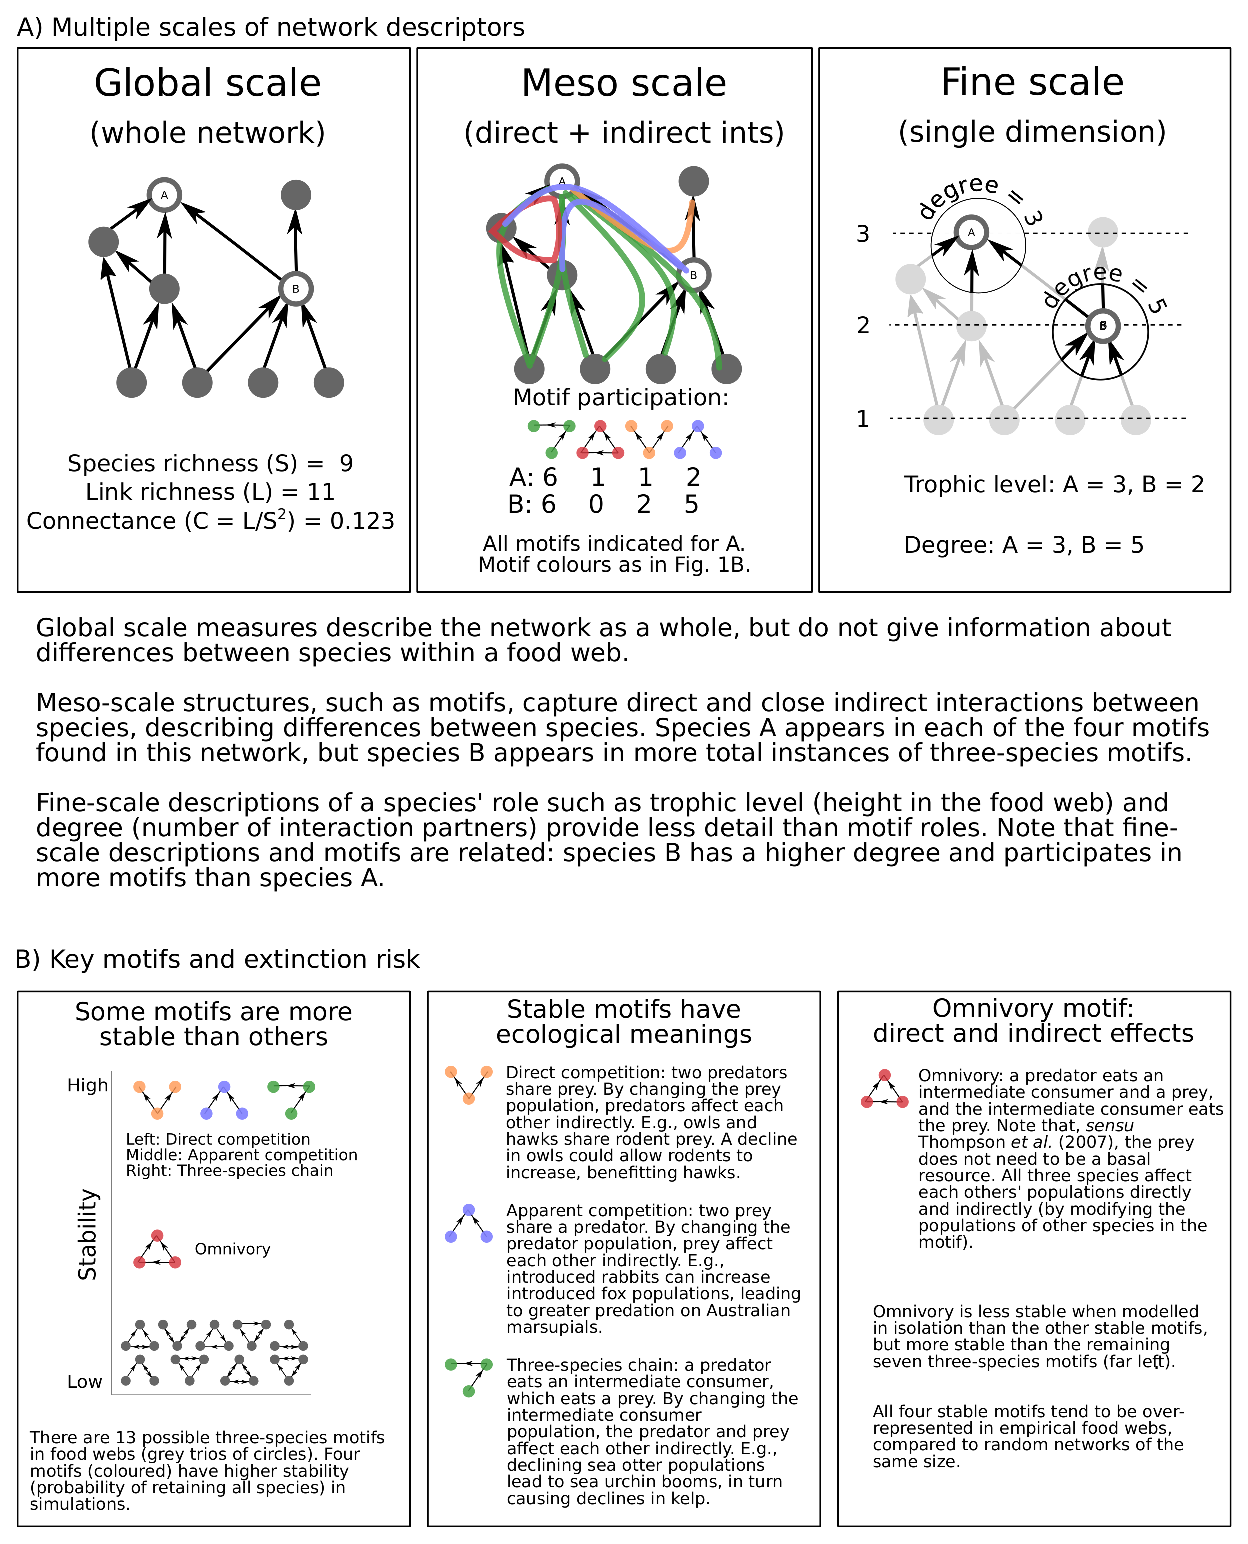
\includegraphics[width=.9\textwidth]{figures/motifs_box.eps}
        \textbf{Figure 1.} A brief introduction to motifs.
        % \label{motifs}
        % \end{figure}

        \vspace{12pt}

   % % PLS coefficients
        % 	\begin{figure}[h!]		
        \noindent \textbf{Figure 2.} Sum of loadings of motif roles, degree, shortest trophic level (STL), web size (S), connectance (C), and their interaction (S:C) in the optimum number of axes in partial least squares regressions of mean time to extinction against all of the above predictors with stable motifs shaded. We fit separate models for: \textbf{A-B)} raw motif counts, \textbf{C-D)} degree-normalized motif frequencies (i.e., proportions of the role made up by each motif) and \textbf{E-F)} network-normalized motif frequencies (i.e., $Z$-scores for each motif compared to all species in the network). 
    	Panels \textbf{A, C, E} (blue) give the sum of loadings for centered, scaled predictors.
    	Panels \textbf{B, D, F} (green) give the sum of loadings from the same models, de-scaled to reflect a unit increase in the predictor.
    	Motif names as in Fig. S3, \emph{Appendix S6}.
        % 		\label{coefficient_sum}
        % 		\includegraphics[height=0.6\textheight]{figures/PLS/total_coefficients.eps}
        % 		\end{figure}


    \vspace{12pt}

    % % Relationships between motifs and degree
% 	\begin{figure}[h!]
	\noindent\textbf{Figure 3.} \textbf{A-B)} Species with more interaction partners or higher trophic levels participated in more motifs, especially the four stable motifs (S1, S2, S4, and S5). 
        \textbf{C)} The proportion of the omnivory motif (S2) increased with increasing degree while those of the other stable motifs decreased. \textbf{D)} The proportions of all four stable motifs  decreased with increasing trophic level.
		\textbf{E)} The $Z$-scores of all motifs increased with increasing degree.
        \textbf{F)} Species with high trophic levels tended to show under-representation of the four stable motifs while unstable motifs could be over- or under-represented. 
        In all panels, motifs are plotted in order of the strength of their relationship with degree and all relationships were significant. 
        Stable motifs (S1, S2, S4, and S5) are indicated by blue or green lines. 
        % 95\% confidence intervals about the regression lines are too small to be visible in the current plot. 
        For motif names see~\citet{Stouffer2007}; Fig. S3, \emph{Appendix S6}.
% 		\label{motif_vs_degTL}
% 		\includegraphics[height=.65\textheight]{figures/roles/motif_vs_oneD.eps}
% 		\end{figure}
\end{spacing}

\clearpage

\section*{Figures}


    \begin{figure}[h!]
        \caption{Figure 1.}
        \label{motifs}
        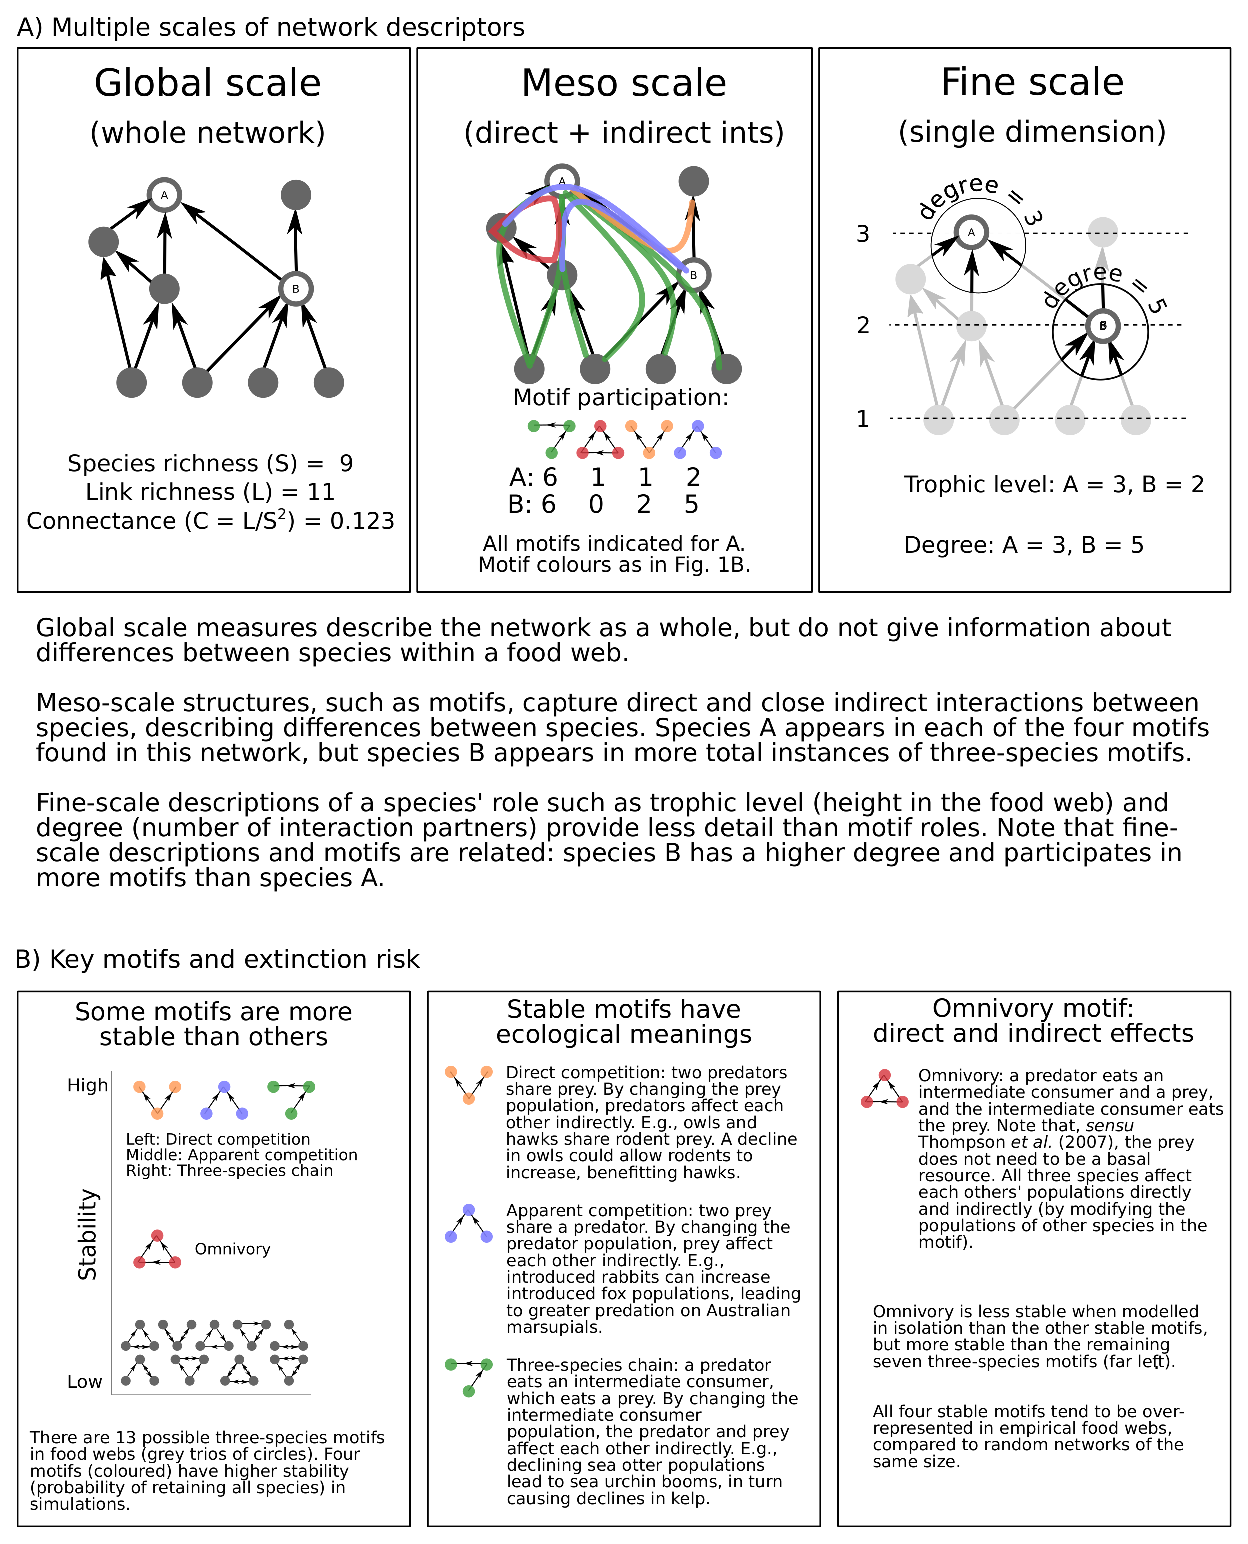
\includegraphics[width=.9\textwidth]{figures/motifs_box.eps}
    \end{figure}

    \clearpage

    % % PLS coefficients
	\begin{figure}[h!]
		\caption{Figure 2.}
        \label{coefficient_sum}
        \includegraphics[height=0.6\textheight]{figures/PLS/total_coefficients.eps}
        \end{figure}

    \clearpage
    
    % % Relationships between motifs and degree
	\begin{figure}[h!]
		\caption{Figure 3.}
        \label{motif_vs_degTL}
        \includegraphics[height=.65\textheight]{figures/roles/motif_vs_oneD.eps}
		\end{figure}


\clearpage

\section*{Appendices}

\begin{spacing}{2.0}

All of the following Appendices are included as supplemental information.

    \subsection*{S1: Details of network generation}

        Supplemental methods describing how the initial networks were generated and population dynamics simulated.

    \subsection*{S2: Testing consistence of times to extinction}
    
        Supplemental methods and results related to testing whether the identity of the removed species has a large effect on the time to extinction for non-removed species. Includes \textbf{Figure S1}.
    
    \subsection*{S3: Details of PERMANOVA methods and results}
        
        Supplemental methods and results for PERMANOVAs testing whether species' overall roles are related to their mean times to extinction. Includes \textbf{Figure S2, Tables S1-S2}.

    \subsection*{S4: Details of PLSR methods}

        Supplemental methods for partial least squares regressions. 
    
    \subsection*{S5: Relating motifs roles to other measures}
        
        Gives the slopes of relationships between motif roles and degree or shortest trophic level (STL) in \textbf{Tables S3-S4}.
        
    \subsection*{S6: Motif labels}
        
        \textbf{Figure S3} illustrates the 13 unique three-species motifs and labels each one according to the naming scheme in~\citet{Stouffer2007}.

\end{spacing}

\end{document}



